
\documentclass[11pt,a4paper,computermodern]{article}


\usepackage[
%	includeheadfoot,
	width=172mm,
	top=18mm,
	bottom=18mm,
	bindingoffset=4mm
	]{geometry}



%%% Typeface packages
\usepackage[utf8]{inputenc}
\usepackage[T1]{fontenc}
\usepackage{fontawesome}

\usepackage{multirow}
\usepackage{tabularx}
\usepackage{booktabs}
\usepackage[flushleft]{threeparttable}
\usepackage{enumitem}

%%% Graphics packages
\usepackage{graphicx}
\usepackage{subcaption}


%%

\usepackage{hyperref}
\hypersetup{
	colorlinks=false,
	hidelinks=true,
}



%%
\title{Spotify Data Landscape}
\date{}


\begin{document}

\maketitle

\vspace{-10mm}

Spotify, founded in 2006 and now serving over 600 million monthly active users globally, including 250 million premium subscribers, is the world’s leading audio streaming platform. Operating in more than 180 countries, Spotify relies heavily on data to deliver personalized experiences, power its recommendation engine, and drive content and marketing strategies. The company manages a vast and complex data ecosystem that includes user behavioral data (e.g., listening habits, search history), content metadata (e.g., song attributes, podcast tags), subscription and billing data, advertising engagement metrics, and localized market insights. This rich data landscape is foundational to the innovation of Spotify but also demands a robust governance framework to ensure data quality, compliance with global privacy regulations like GDPR and CCPA, and secure, ethical use of user information.


\section*{Data Maturity Assessment}

Spotify must adapt its data governance to the constraints imposed by its rapid growth. We provide in this section a comprehensive assessment of its maturity for each of the knowledge areas of the DAMA-DMBoK data management framework.

\begin{figure}[ht]
	\begin{subfigure}[h]{0.4\linewidth}
		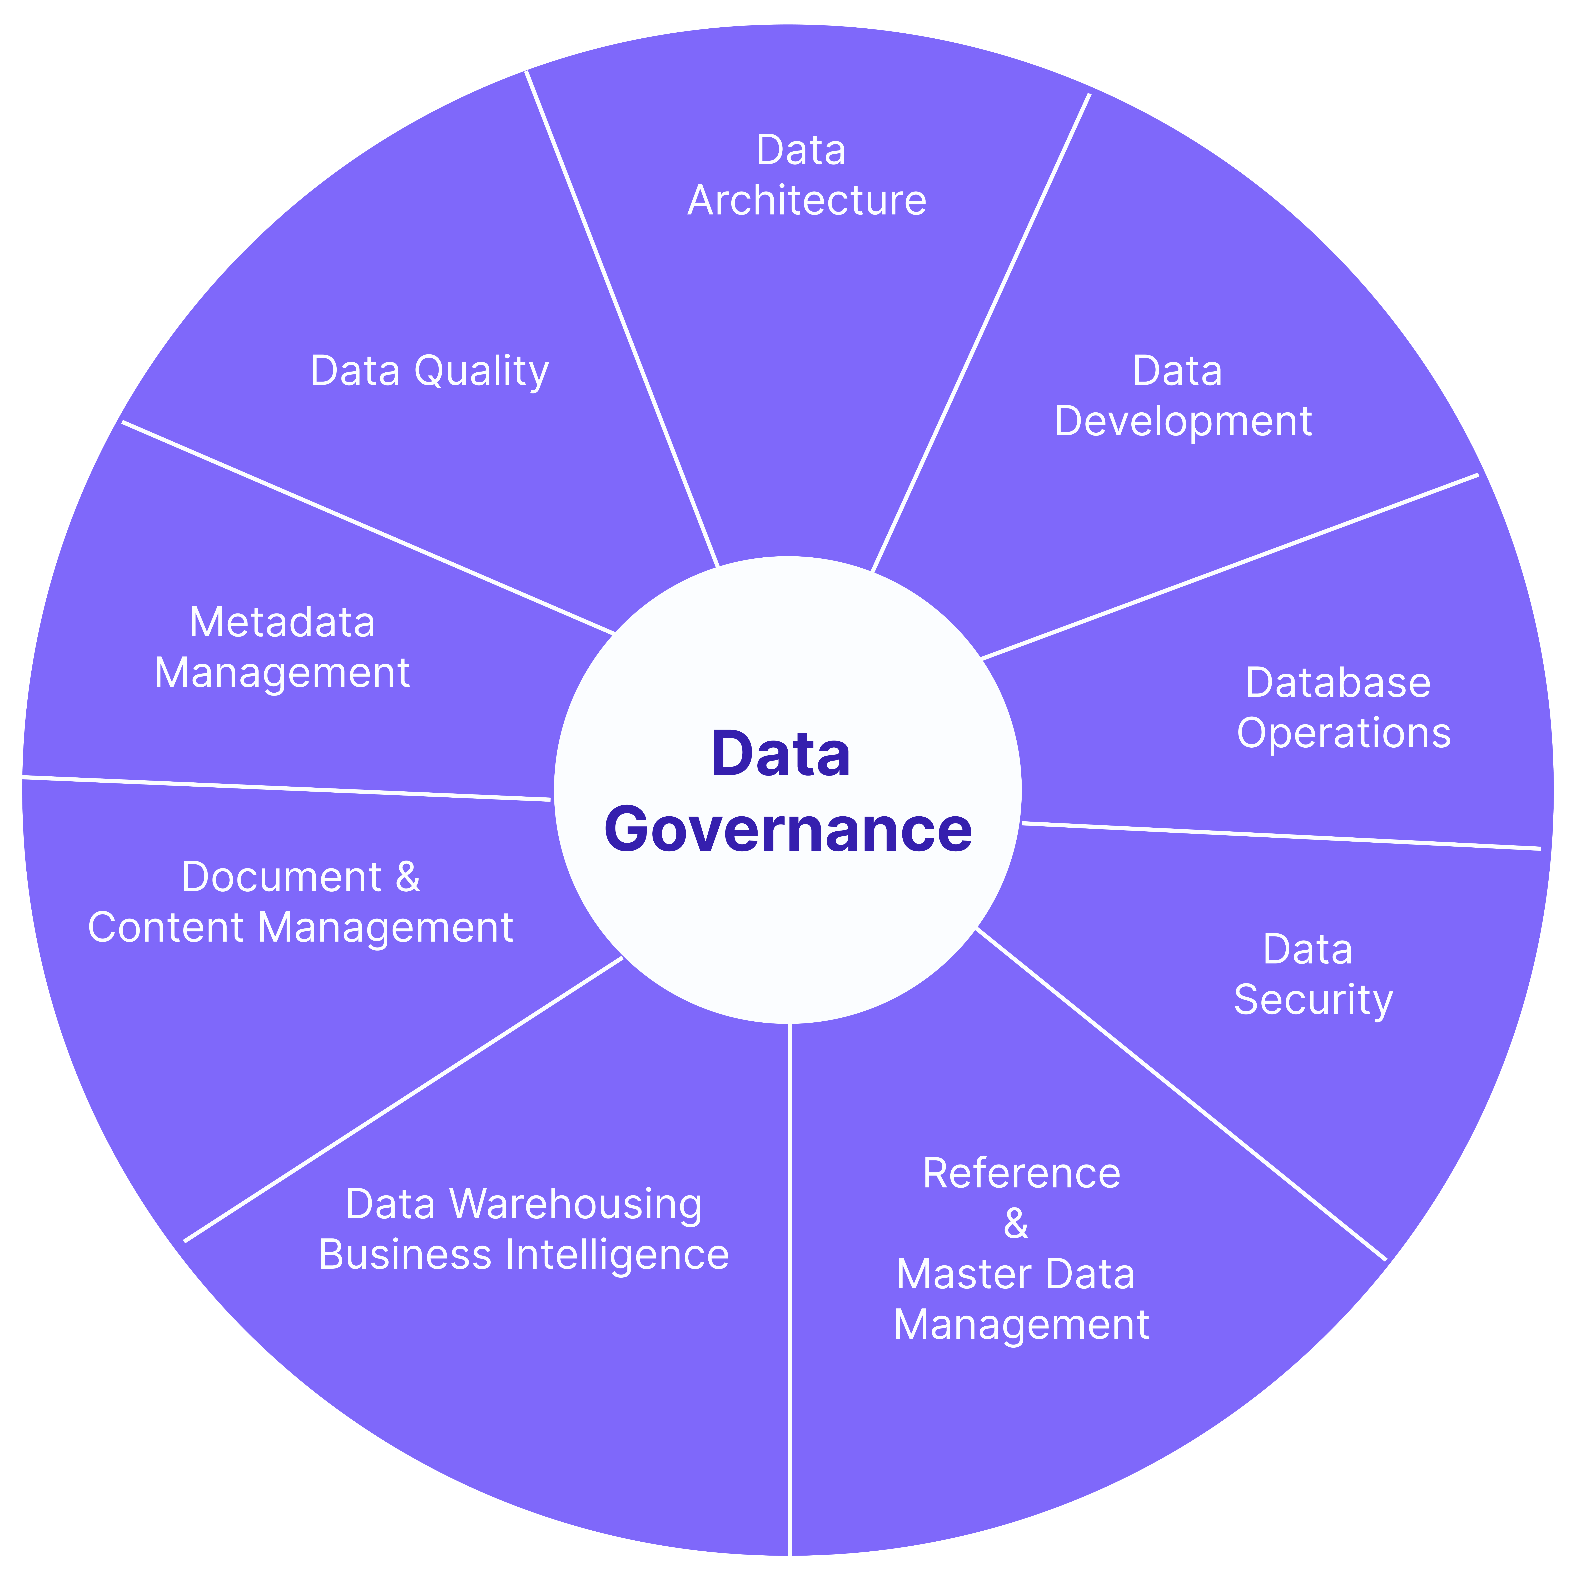
\includegraphics[width=\linewidth]{./figures/DMBoK_v3}
	\end{subfigure}
	\hfill
	\begin{subfigure}[h]{0.58\linewidth}
		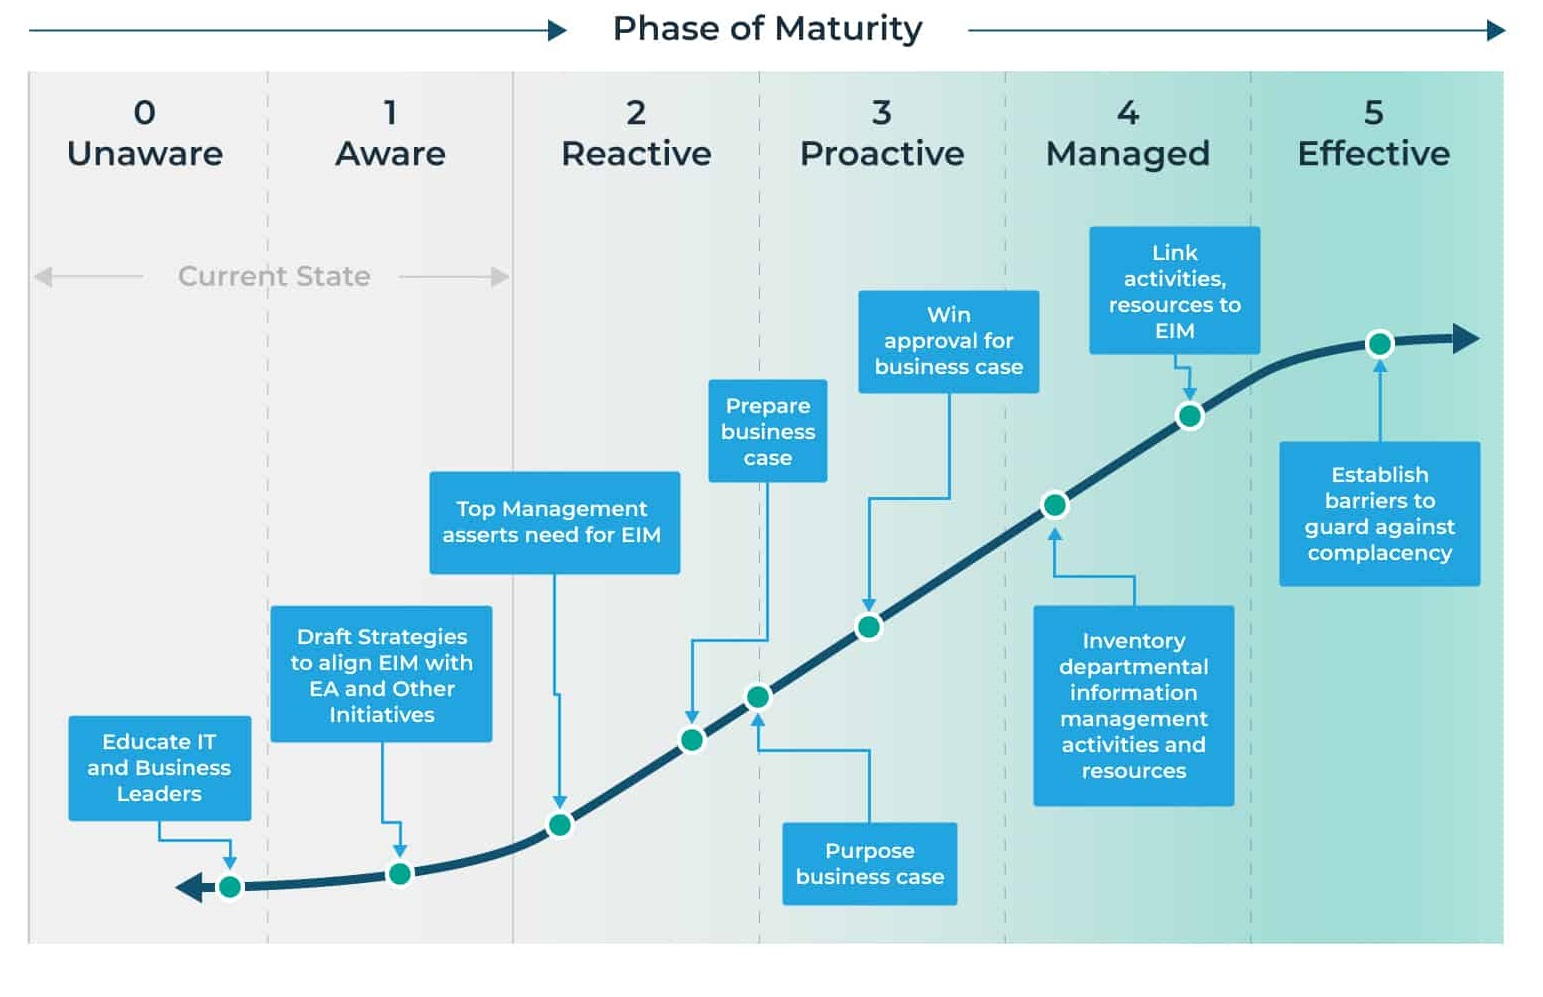
\includegraphics[width=\linewidth]{./figures/data_maturity}
	\end{subfigure}
%	%\caption{Proposed OLTP database structure.}
	\label{fig:DataManagement}
\end{figure}

\begin{itemize}[itemsep=5pt, parsep=0pt]
	\item \textbf{Data Governance: level 2 - Reactive}\\
	No unified governance framework exists; data ownership and stewardship are informal and siloed.
	\item \textbf{Data Architecture: level 3 - Proactive}\\
	Sophisticated architecture using cloud, lakes, and databases, but lacks enterprise-wide integration and standardization.
	\item \textbf{Data Development: level 3 - Proactive}\\
	Strong ML and engineering capabilities, but development practices are fragmented with inconsistent documentation.
	\item \textbf{Data Operations Management: level 3 - Proactive}\\
	Real-time data pipelines are robust, but operational monitoring and SLAs are inconsistent across teams.
	\item \textbf{Data Security Management: level 4 - Managed}\\
	Advanced controls are in place, but evolving regulatory environments create ongoing compliance risks.
	\item \textbf{Reference and Master Data Management: level 2 - Reactive}\\
	Artist, content, and user master data are inconsistently managed across departments, leading to duplication.
	\item \textbf{Data Warehousing and Business Intelligence Management: level 3 - Proactive}\\
	Analytics infrastructure is powerful but suffers from limited cross-team visibility and fragmented key performance indicators.
	\item \textbf{Document and Content Management: level 2 - Reactive}\\
	No centralized taxonomy or governance for podcast metadata, contracts, or localized content documentation.
	\item \textbf{Meta-data Management: level 2 - Reactive}\\
	Inconsistent metadata practices and lack of a centralized data catalog hinder discoverability and quality.
	\item \textbf{Data Quality Management: level 2 - Reactive}\\
	Data quality is reactive; missing validation processes and automated cleansing across data pipelines.
	\item \textbf{Data Compliance: level 3 - Proactive}\\
	Active GDPR/CCPA efforts, but no unified compliance framework; needs structured oversight and audits.
	\item \textbf{Data Literacy: level 2 - Reactive}\\
	Data usage varies by team; limited formal training and a strong reliance on technical staff for interpretation.
\end{itemize}


\section*{Key Governance Challenges}

The growth and innovation of Spotify depend on turning its advanced data infrastructure into a well-governed, integrated, and trusted data ecosystem. This will require formalizing data governance policies, building roles like Data Stewards, and establishing foundational practices in metadata, quality, and literacy — all while maintaining compliance in a complex global regulatory environment.

\begin{itemize}[itemsep=5pt, parsep=0pt]
	\item \textbf{Data silos and fragmentation}\\
	Independent data handling by departments like marketing, product, and engineering leads to inconsistent, incomplete data views and hinders unified analytics.
	\item \textbf{Regulatory Compliance Complexity}\\
	Navigating diverse regulations (GDPR, CCPA) across more than 180 countries requires a dynamic compliance strategy and stronger oversight.
	\item \textbf{Low metadata quality and standards}\\
	Metadata is inconsistently applied, and data quality issues negatively impact core systems like the recommendation engine.
	\item \textbf{Access and integration barriers}\\
	Disconnected systems delay innovation and product launches; employees lack timely access to needed data.
	\item \textbf{User privacy and trust}\\
	Increasing user awareness of data rights demands greater transparency, consent management, and anonymization protocols.
	\item \textbf{Weak data culture}\\
	While data is critical to strategy, there is limited enterprise-wide literacy, governance awareness, or data stewardship.
\end{itemize}


\end{document}